
\section{A fresh approach for Structural Bioinformatics: \biochem}
\label{sec:juliaball}
In this work, we sought to redesign the popular \ball package for molecular analysis and simulation. This section initially examines reasons for a redesign in Julia, followed by a description of the core implementation of \biochem closing with the benchmark results. 

\subsection{Reasons for a redesign or \textit{why Julia?}}

While the design goals and the need for an open-source framework with the rich functionality such as \ball's  is still present, the realization of the main design principles of \ball are highly dependent on the choice of the programming language. From today's perspective in particular with regard to its purpose as a platform for rapid application development~(RAD), the usage of C++ may be considered suboptimal. \\
As for many scientific software packages, the development times for applications play a crucial role for the acceptance and usability of the underlying software. For example, a great deal of time may have to be spend by installing the library with its dependencies. Although the CMake build system has been integrated in version 1.3, setting up the library is a highly non-trivial task. Additionally, the development times are massively influenced by the knowledge of the used programming language. As a low-level language, C++ is known to require more time to be learned compared to scripting languages such as Python \cite{Ousterhout1998}. 
Even with the additional Python bindings, the integration of new functionality is still not straightforward. In contrast, the implementation of new features is typically associated with the addition of massive amounts of boilerplate code. This applies to an even greater extent, in cases where portability to different platforms and compiler settings have to be supported. \\
Consequently, \ball itself can be considered as a textbook example for the two language problem, which is very common for scientific computing project. In the latter, the core functionality is often implemented in a low-level programming language, ensuring the required performance, while higher-level programming languages are used for user-friendly interfaces to the core functionalities. Julia is exactly developed for these situations \cite{Julia_what, Julia_accomplish}.\\ Nevertheless, it is important to keep in mind, that back in 1996 and still in 2010, C++ was the best choice for the implementation of \ball. \\
The design goals as described in the previous section are achieved in a much easier way with the usage of Julia:
\begin{itemize}
	\item ease of use: Julia is easier to learn and ideas can be implemented from scratch. The times to inter, installation and portability, documentation is integrated
	\item Openness: integration of external tools trivial, 
	\item robustness: \biochem has been developed with accompanying test case for the core structures as well as for the functionalities, benchmarks have been implemented to ensure performance, both things were integrated on the fly
	\item functionality, not yet feature complete but we can already do things as described in the applications section
\end{itemize}


\subsection{The core}
In addition to the four original design goals, we sought to make \biochem comparable in performance to \ball. The core data structures play key roles in the efficiency of the entire framework. When working with structural data of molecular entities such as proteins, or nucleic acid molecules (DNA/RNA), the representation of three dimensional coordinates play an important role. 

Just like in \ball we define a similar hierarchical structure...as can be seen in fig..
Optimized for random access to any atoms...
same hand easy to use for Julia users or Python users familiar with Pandas DataFrames...
So initially, representation was based on DataFrames. While theis is extremely intuitive, it has some 


\begin{figure*}[t]
	\centerline{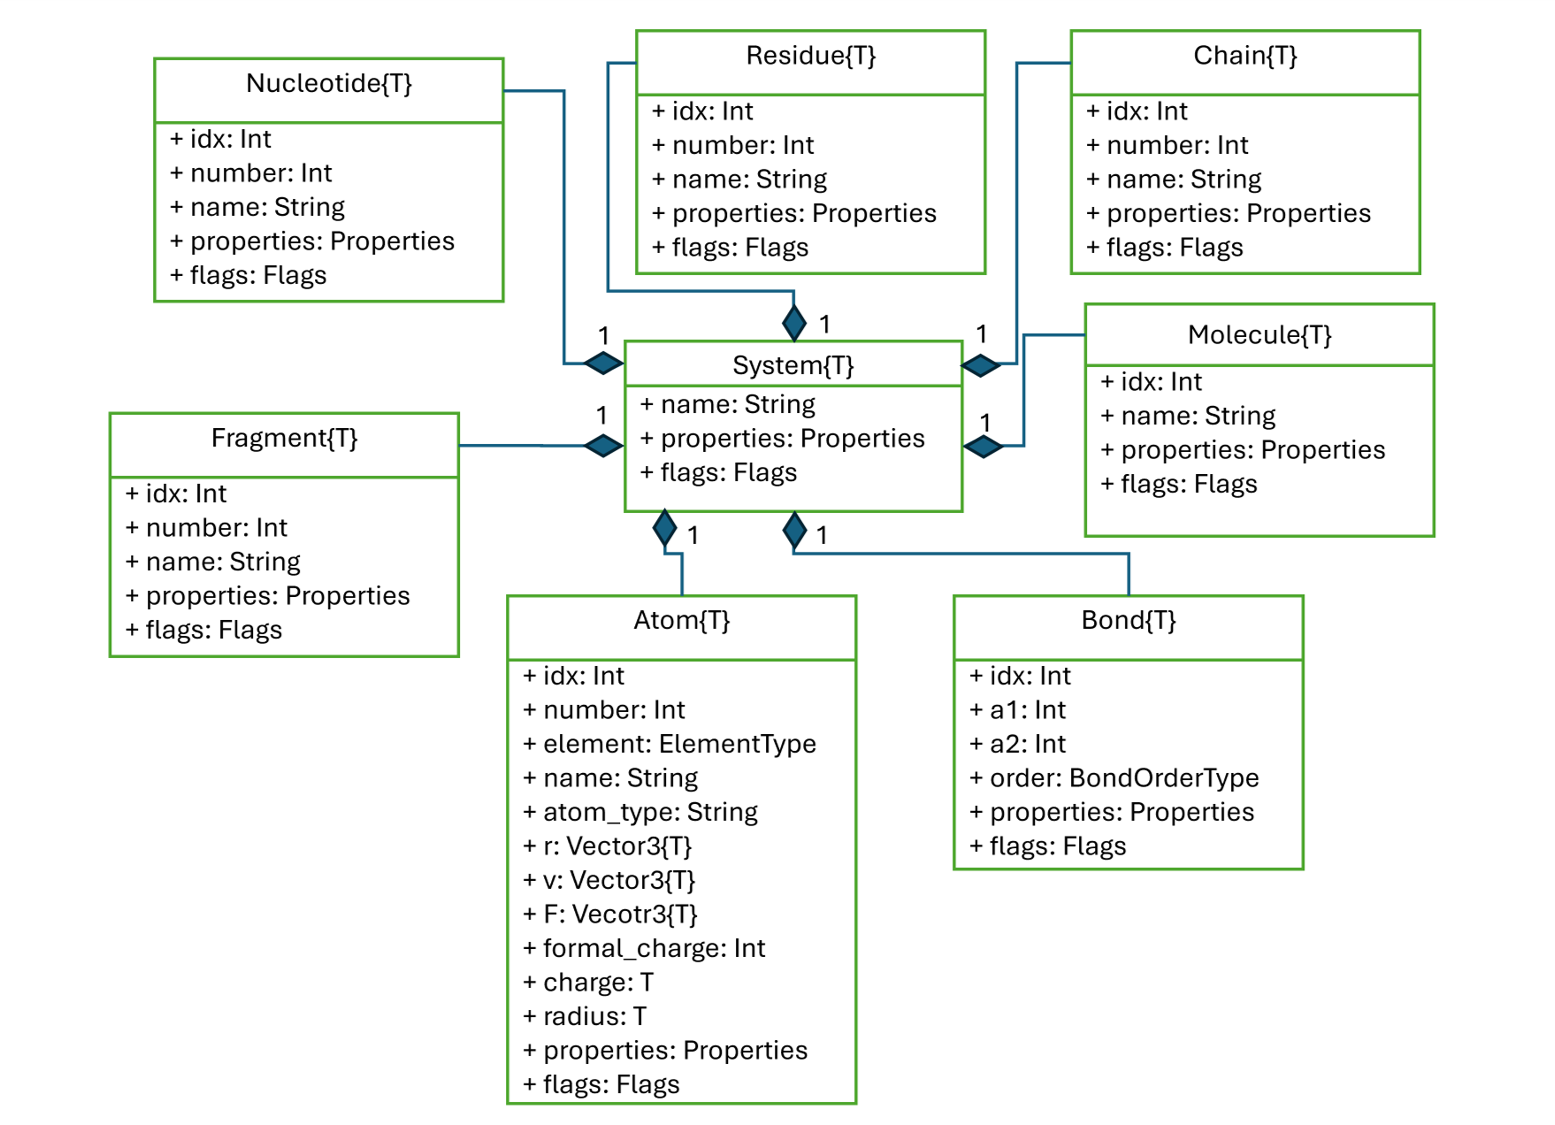
\includegraphics[width=15cm]{gfx/uml.png}}
	\caption{UML-Diagramm of the core of \biochem . In the center resides the \texttt{System} interface. All other functionalities are grouped around that core piece. Only the most important functionalities of each class are  shown.}
	\label{fig:biochem_uml}
\end{figure*}

\subsection{Benchmarks}
On par with its C++ predecessor
it is intuitiv to write code that is 

\begin{table}
	\tbl{Example tasks and the required time}{
		\begin{tabular}{|l|c|c|}\hline
			Description & \ball & \biochem \\
			tba & tba & tba\\hline
			tba & tba & tba \\\hline
		tba	& tbal & tba \\ \hline
	\end{tabular}}
\end{table}